\hypertarget{fast-axis-collimator-facet-loss-relay-lens-and-the-power-plan}{%
\chapter{Fast-axis collimator, facet loss, relay lens and the power
plan}\label{collimator-fast-axis-collimator-facet-loss-relay-lens-and-the-power-plan}}

\begin{quote}
Follow-up (\texttt{docs/megascale.md}, Sec. 12): this module and
\texttt{docs/stacked\_relay.md} treat the y axis for light with no x
component (s\_x = 0). A tweezer at x\_a is made of light with s\_x =
x\_a / 288 um, and the cylindrical collimator then acts with effective
indices sqrt(n\^{}2 - s\_x\^{}2). The adopted collimator defocuses the
facet by -99 s\_x\^{}2 um. The y figures below therefore hold near the
row centre: the peak falls to 0.97 at x\_a = 30 um and 0.48 at 60 um.
With the best common focus offset a row is usable over
\textbar x\_a\textbar{} \textless= 45 um.

Follow-up (Sec. 10, module 27): an all-reflective collimator removes
this limit. Two mirrors in one fused-silica block glued to the facet
collimate exactly at every s\_x and obey the sine condition. In 1D the
peak stays at or above 0.98 out to the slit edge (x\_a = 102 um), and
the on-axis figures equal those of the refractive design. The costs are
a mirror form tolerance of about 10 nm rms (against 20 nm) and
coating-dependent polarisation (Sec. 10.5).
\end{quote}

Follow-up to \texttt{docs/stacked\_relay.md}, which assumed an ideal
collimator (focal length 175 um, NA 0.9, Abbe sine condition). Code:
\texttt{picsim/raytrace.py}, \texttt{picsim/opa/collimator.py},
\texttt{scripts/m14\_collimator.py},
\texttt{scripts/m14\_facet\_meep.py} (2D FDTD); results
\texttt{results/m14\_*.json}. Values are SIM or DERIVED, valid in the
regime stated. They should be reviewed before they are quoted.

\hypertarget{1-result}{%
\section{Result}\label{collimator-1-result}}

A collimator that meets the requirement exists in a classical form. It
is an aplanatic (Weierstrass) cylinder on a fused-silica block glued to
the facets, followed 10 um later by a two-asphere aplanat of index 1.8.
Ray traced, it collimates to NA 0.9 with the sine condition exact and no
residual wavefront error. Rays meet every surface at 25 deg or less, and
the whole lens is 0.40 mm long and 0.32 mm tall. In the wave model it
performs like the ideal lens in glass. Two findings change the system
numbers:

(i) \textbf{The emitter facet loses about a quarter of the light into
air.} A 2D FDTD of the facet cross-section gives 79\% transmission into
air (12.8\% reflected back into the chip) and 96\% into glass (2.3\%
reflected). Within the collimator aperture (\textbar s\textbar{}
\textless{} 0.9) the figures are 77\% (air) and 85\% (glass). This loss
was not in any earlier power figure. Gluing the collimator to the facet
recovers about 10\% and cuts the back-reflection sixfold.

(ii) \textbf{Power per 1.2 mK tweezer rises to 57 mW} with the adopted
collimator, from 47 mW (\texttt{docs/stacked\_relay.md}, facet loss
omitted). With an ideal lens in air it would be 61 mW.

{\small
\begin{longtable}[]{@{}>{\raggedright\arraybackslash}p{0.556\dimexpr(\linewidth-4\tabcolsep)\relax}>{\raggedright\arraybackslash}p{0.444\dimexpr(\linewidth-4\tabcolsep)\relax}@{}}
\toprule\noalign{}
quantity & adopted collimator (Weierstrass block + aplanat) \\
\midrule\noalign{}
\endhead
\bottomrule\noalign{}
\endlastfoot
focal length / NA / sine-condition error over the aperture & 175 um /
0.9 / \textless{} 4e-5 \\
length (facet to last vertex) / clear height & 395 um / +/-158 um \\
largest incidence angle on any surface & 25 deg \\
peak per guided power vs ideal lens in air & 1.10 (2D check: 1.107) \\
row crosstalk at 4 um (1D line; 2D single tweezer 1.7e-4) & 8.4e-5 \\
decentre / focus for \textless= 3\% loss (1D line; in 2D: 0.988 / 0.953
at 0.5 / 1 um focus, 0.968 at 0.1 um decentre) & +/-0.1 um / +/-1 um \\
surface form error for \textless= 2\% loss & \textless= 20 nm rms \\
laser power per 1.2 mK tweezer & 57 mW \\
\end{longtable}
}

The decentre tolerance (+/-0.1 um) does not depend on the lens design.
It is set by the small vertical mode of the facet. The first x lens of
the relay, by contrast, needs no special accuracy, because calibration
absorbs its static aberration (Sec. 6). One HI1060-matched input fibre
per chip carries the 2.6 to 3.4 W a row needs, at 7 to 9 MW/cm\^{}2
(Sec. 8).

\hypertarget{2-why-na-09-at-175-um-is-hard}{%
\section{Why NA 0.9 at 175 um is
hard}\label{collimator-2-why-na-09-at-175-um-is-hard}}

A collimator must bend rays from sin(theta) = 0.9 (64 deg in air) to the
axis within a lens no taller than the 0.5 mm chip pitch. Single
refracting surfaces fail:

(i) a plano-hyperbolic lens with its curved side to the facet collimates
exactly, but only up to sin(theta) = sqrt(1 - 1/n\^{}2): 0.72 for fused
silica and 0.83 for n = 1.8; (ii) a plano-asphere with its flat side to
the facet reaches 0.9. In fused silica its exit surface slopes at 81 deg
and rays meet it at 43 deg, at the edge of total internal reflection.
With n = 1.8 the slope falls to 58 deg, but the flat surface then sees
64 deg incidence (51\% bare transmission), which an AR coating cannot
easily recover; (iii) one elliptical surface on a block glued to the
facet (source inside glass, eccentricity 1/n) collimates exactly at any
NA up to sqrt(n\^{}2 - 1) = 1.05. However, it violates the sine
condition: the ray at s = 0.9 exits at 68\% of the height an aplanatic
lens would give.

The Weierstrass construction resolves this. A circular surface (radius
R) on a glass block, with the facet R/n from its centre, is aplanatic:
every ray appears to come without aberration from a virtual point, and
the NA drops by n\^{}2 (0.9 -\textgreater{} 0.43 for fused silica). A
second lens of focal length f n\^{}2 = 368 um then collimates NA 0.43.
We design it as a two-asphere aplanat in 2D (Wassermann-Wolf
construction: exact collimation and exact sine condition,
\texttt{collimator.aplanat}). A scan of R, the air gap, the aplanat
thickness and its index (96 combinations, 29 reaching NA 0.9;
\texttt{m14\_scan}) selected R = 80 um, a 10 um gap, a 250 um thick
aplanat and n = 1.8. That combination gives the lowest largest incidence
angle (25.4, 18.2 and 19.2 deg on the three surfaces) and slopes of 64,
7 and 36 deg.

{\footnotesize
\begin{longtable}[]{@{}>{\raggedright\arraybackslash}p{0.219\dimexpr(\linewidth-10\tabcolsep)\relax}>{\raggedright\arraybackslash}p{0.270\dimexpr(\linewidth-10\tabcolsep)\relax}>{\raggedright\arraybackslash}p{0.140\dimexpr(\linewidth-10\tabcolsep)\relax}>{\raggedright\arraybackslash}p{0.157\dimexpr(\linewidth-10\tabcolsep)\relax}>{\raggedright\arraybackslash}p{0.213\dimexpr(\linewidth-10\tabcolsep)\relax}@{}}
\toprule\noalign{}
design & sine condition y\_S/(f s) at s = 0.3 / 0.6 / 0.9 & largest
incidence & surfaces & Fresnel transmission at the edge, bare \\
\midrule\noalign{}
\endhead
\bottomrule\noalign{}
\endlastfoot
Weierstrass + aplanat (glued) & 1.000 / 1.000 / 1.000 & 25 deg & 3 (one
spherical) & 0.74 \\
ellipse (glued or printed) & 0.954 / 0.834 / 0.675 & 43 deg & 1 &
0.43 \\
plano-asphere, n = 1.8 (air) & 0.988 / 0.960 / 0.971 & 64 deg & 2 &
0.51 \\
\end{longtable}
}

\hypertarget{3-facet-transmission}{%
\section{Facet transmission}\label{collimator-3-facet-transmission}}

The x model of the chip treated the emitter facet as lossless, and the
cross-axis model of module 13 normalised to the power radiated into air.
A Kirchhoff estimate puts the loss into air at 27\%. It comes from 8\%
Fresnel reflection plus the 20\% of the angular spectrum of the 0.39 um
vertical mode that lies beyond the light cone. We checked this by 2D
FDTD (MEEP, resolution 40/um) of the vertical cross-section. The SiN
core index was set to 1.965 so that the slab mode index equals that of
the 3D mode (1.7995). The guide ends in air, or in fused silica for a
glued lens.

{\small
\begin{longtable}[]{@{}>{\raggedright\arraybackslash}p{0.121\dimexpr(\linewidth-10\tabcolsep)\relax}>{\raggedright\arraybackslash}p{0.189\dimexpr(\linewidth-10\tabcolsep)\relax}>{\raggedright\arraybackslash}p{0.227\dimexpr(\linewidth-10\tabcolsep)\relax}>{\raggedright\arraybackslash}p{0.273\dimexpr(\linewidth-10\tabcolsep)\relax}>{\raggedright\arraybackslash}p{0.189\dimexpr(\linewidth-10\tabcolsep)\relax}@{}}
\toprule\noalign{}
into & reflected & transmitted & within the collimator aperture, FDTD &
same, Kirchhoff \\
\midrule\noalign{}
\endhead
\bottomrule\noalign{}
\endlastfoot
air & 12.8\% & 79.1\% & 77.2\% & 72.3\% \\
fused silica & 2.3\% & 95.9\% & 85.2\% & 82.9\% \\
\end{longtable}
}

The two methods agree to 3 to 7\%. We use the FDTD values to scale the
Kirchhoff spectra in the power estimate. The remainder (8\% in air, 2\%
in glass) leaves through the cladding near the facet. It is a 2D result
with the lateral confinement folded into the core index; a 3D FDTD of
the facet would refine it.

\hypertarget{4-the-designs-in-the-wave-model}{%
\section{The designs in the wave
model}\label{collimator-4-the-designs-in-the-wave-model}}

The wave model takes the facet spectrum in air or glass, each
lens\textquotesingle s traced map (exit height and wavefront vs s,
Fresnel transmission), the pupil fill beta and the NA 0.5 pupil. Peak
values are per unit guided power, relative to the ideal lens in air at
beta = 0.7 um, with AR-coated lens surfaces:

{\small
\begin{longtable}[]{@{}>{\raggedright\arraybackslash}p{0.383\dimexpr(\linewidth-10\tabcolsep)\relax}>{\raggedright\arraybackslash}p{0.117\dimexpr(\linewidth-10\tabcolsep)\relax}>{\raggedright\arraybackslash}p{0.117\dimexpr(\linewidth-10\tabcolsep)\relax}>{\raggedright\arraybackslash}p{0.117\dimexpr(\linewidth-10\tabcolsep)\relax}>{\raggedright\arraybackslash}p{0.266\dimexpr(\linewidth-10\tabcolsep)\relax}@{}}
\toprule\noalign{}
design & beta & peak & y FWHM & crosstalk at 3 / 4 um \\
\midrule\noalign{}
\endhead
\bottomrule\noalign{}
\endlastfoot
ideal, air & 0.7 um & 1.00 & 1.31 um & 2.8e-4 / 1.1e-4 \\
\textbf{Weierstrass + aplanat} & 0.7 um & \textbf{1.10} & 1.35 um &
4.0e-4 / 8.4e-5 \\
ellipse, printed & 0.9 um & 1.03 & 1.35 um & 6.6e-4 / 1.8e-4 \\
ellipse, printed & 0.7 um & 1.22 & 1.13 um & 2.1e-3 / 1.0e-3 \\
plano-asphere n = 1.8 & 0.7 um & 1.03 & 1.27 um & 4.0e-4 / 1.7e-4 \\
\end{longtable}
}

The aplanatic design reproduces the ideal lens in glass exactly. The
ellipse narrows the y spot because its mapping compresses the outer far
field, but the same distortion raises the crosstalk. Opening the pupil
fill to beta = 0.9 um restores 1.8e-4 at 4 um at a cost of 15\% in peak.
Without AR coatings, all designs lose 10 to 30\% (n = 1.8 surfaces
reflect 8\% each at normal incidence), so coatings are needed in every
case.

\hypertarget{5-tolerances-with-the-real-lenses}{%
\section{Tolerances with the real
lenses}\label{collimator-5-tolerances-with-the-real-lenses}}

{\footnotesize
\begin{longtable}[]{@{}>{\raggedright\arraybackslash}p{0.310\dimexpr(\linewidth-10\tabcolsep)\relax}>{\raggedright\arraybackslash}p{0.103\dimexpr(\linewidth-10\tabcolsep)\relax}>{\raggedright\arraybackslash}p{0.207\dimexpr(\linewidth-10\tabcolsep)\relax}>{\raggedright\arraybackslash}p{0.131\dimexpr(\linewidth-10\tabcolsep)\relax}>{\raggedright\arraybackslash}p{0.248\dimexpr(\linewidth-10\tabcolsep)\relax}@{}}
\toprule\noalign{}
error & ideal (air) & Weierstrass + aplanat & ellipse & plano-asphere n
1.8 \\
\midrule\noalign{}
\endhead
\bottomrule\noalign{}
\endlastfoot
decentre 0.1 / 0.2 um & 0.973 / 0.897 & 0.973 / 0.896 & 0.962 / 0.855 &
0.971 / 0.887 \\
focus 0.5 / 1 um & 0.989 / 0.937 & 0.995 / 0.977 & 0.974 / 0.905 & 0.978
/ 0.906 \\
form error 20 / 50 nm rms (corr. 20 um), mean & & 0.984 / 0.916 & 0.998
/ 0.988 & 0.989 / 0.916 \\
form error 50 nm, 10th percentile & & 0.880 & 0.981 & 0.865 \\
\end{longtable}
}

(Peak relative to no error, 1D y line, beta = 0.7 um for all designs.)

The tolerance model was checked against exact traces of a displaced
source. For decentres of 0.2 and 0.5 um and a 0.5 um focus error, the
exactly traced path change differs from the first-order model by at most
0.003 waves rms (0.03 waves peak-to-valley for the ellipse at 0.5 um,
about 2e-4 waves for the aplanatic design).

Three points follow. (i) The decentre tolerance is a property of the
facet, not of the lens: +/-0.1 um for every design. (ii) Focus is looser
for the glued designs because the facet radiates into glass (the defocus
phase scales as n\_m cos theta): about +/-1 um for 3\%. (iii) The
ellipse has one surface with a small index step (n - 1 = 0.45), so it
tolerates 50 nm rms form error; the n = 1.8 surfaces need about 20 nm.

\hypertarget{6-the-first-x-lens-of-the-relay}{%
\section{The first x lens of the
relay}\label{collimator-6-the-first-x-lens-of-the-relay}}

The x relay\textquotesingle s first lens (f = 3.12 mm, NA 0.355 through
the slit) sees the whole emitter row, +/-144 um, so it works off axis.
We traced two fused-silica designs from 7 emitter heights. Each off-axis
wavefront was applied to each emitter\textquotesingle s angular spectrum
in the D1 model (BPM matrix), and tweezers at 0, +/-30 and +/-60 um were
evaluated before and after least-squares recalibration. (Corrected: the
first aplanat, with r0 = 1.5 mm, covered only \textbar s\textbar{}
\textless= 0.33, short of the slit edge 0.355, and the wavefronts were
quoted at the 125 um field point; the aplanat now uses r0 = 2.0 mm,
which covers the slit at every field point, and both lenses are
evaluated at 144 um. Its back focal distance is 6.76 mm.)

{\footnotesize
\begin{longtable}[]{@{}>{\raggedright\arraybackslash}p{0.191\dimexpr(\linewidth-10\tabcolsep)\relax}>{\raggedright\arraybackslash}p{0.213\dimexpr(\linewidth-10\tabcolsep)\relax}>{\raggedright\arraybackslash}p{0.213\dimexpr(\linewidth-10\tabcolsep)\relax}>{\raggedright\arraybackslash}p{0.229\dimexpr(\linewidth-10\tabcolsep)\relax}>{\raggedright\arraybackslash}p{0.154\dimexpr(\linewidth-10\tabcolsep)\relax}@{}}
\toprule\noalign{}
lens & wavefront at 144 um field (tilt removed) & edge tweezer,
uncalibrated: peak / shift & after recalibration: peak per power / shift
& moving tweezer, others\textquotesingle{} change \\
\midrule\noalign{}
\endhead
\bottomrule\noalign{}
\endlastfoot
aplanat (sine condition), r0 2.0 mm & 0.12 waves rms & 0.983 / 21 nm &
0.998 / \textless= 1.3 nm & 4e-4 / \textless{} 1 nm \\
plano-asphere (no sine condition) & 0.76 waves rms & 0.672 / 590 nm &
0.964 / \textless= 0.5 nm & 4e-4 / 0.7 nm \\
\end{longtable}
}

The static aberration of the x relay is a fixed linear transformation of
the chip\textquotesingle s response. The least-squares synthesis, which
already works on the measured response matrix, removes it. Hence the x
relay needs ordinary lens quality: an aplanat costs nothing, and even a
lens without the sine condition costs only 3.6\%. The same argument does
not apply to the collimator, because the y axis has no actuators.

\hypertarget{7-assembly-and-drift}{%
\section{Assembly and drift}\label{collimator-7-assembly-and-drift}}

(DERIVED, with RECALLED coefficients marked.)

\textbf{Thermal.} For a collimator glued directly onto its own facet,
vertical registration is fixed at the facet. Differential expansion then
acts only over the lens\textquotesingle s own height (+/-80 um at the
glued block): with Delta alpha \textasciitilde{} 2e-6/K (Si 2.6e-6/K vs
fused silica 0.55e-6/K, RECALLED), that is about 0.2 nm/K, negligible. A
monolithic collimator array for the whole stack, referenced at its base,
would see the full 8 mm stack height: 16 nm/K at the top chip, so 0.1 um
after 6 K. Hence one collimator per chip, or a stack held to +/-1 K.

\textbf{Adhesive.} The glue line of the immersed design lies between the
facet and the block, along z. Shrinkage during cure therefore changes
the focus, which tolerates about +/-1 um, and only weakly the decentre.
The vertical position must be held during cure to +/-0.1 um. Typical
shrinkage and creep of UV adhesives need checking {[}REF?{]}.

\textbf{Alignment signal.} Decentre moves the facet image across the
pupil by delta x 12,400 (\texttt{docs/stacked\_relay.md}, Sec. 2): 0.1
um becomes 1.2 mm on the 17 mm pupil. Imaging the pupil, or its
conjugate in the y telescope, while each chip is lit gives a direct and
very sensitive alignment signal. A camera with 10 um pixels resolves 1
nm of decentre in principle. Active alignment against this signal,
before and during cure, is the recommended process. A collimator printed
by two-photon lithography directly on the facet would be registered
lithographically; its placement accuracy needs a source {[}REF?{]}.

\hypertarget{8-power-and-frequency-plan-for-16-chips}{%
\section{Power and frequency plan for 16
chips}\label{collimator-8-power-and-frequency-plan-for-16-chips}}

Laser power per 1.2 mK tweezer, field mean, per unit guided power
(FDTD-scaled facet, AR-coated lenses):

{\small
\begin{longtable}[]{@{}ll@{}}
\toprule\noalign{}
collimator & power per tweezer \\
\midrule\noalign{}
\endhead
\bottomrule\noalign{}
\endlastfoot
ideal lens in air & 61 mW \\
Weierstrass + aplanat, glued (adopted) & 57 mW \\
ellipse, printed, beta 0.9 & 61 mW \\
plano-asphere n = 1.8 in air & 59 mW \\
\end{longtable}
}

{\small
\begin{longtable}[]{@{}>{\raggedright\arraybackslash}p{0.186\dimexpr(\linewidth-10\tabcolsep)\relax}>{\raggedright\arraybackslash}p{0.119\dimexpr(\linewidth-10\tabcolsep)\relax}>{\raggedright\arraybackslash}p{0.119\dimexpr(\linewidth-10\tabcolsep)\relax}>{\raggedright\arraybackslash}p{0.119\dimexpr(\linewidth-10\tabcolsep)\relax}>{\raggedright\arraybackslash}p{0.458\dimexpr(\linewidth-10\tabcolsep)\relax}@{}}
\toprule\noalign{}
tweezers per row & depth & power per chip & 16 chips & input fibres per
chip: lensed tip / HI1060-matched tip \\
\midrule\noalign{}
\endhead
\bottomrule\noalign{}
\endlastfoot
45 (4 um) & 1.2 mK & 2.6 W & 41 W & 5 / 1 (7 MW/cm\^{}2) \\
60 (3 um) & 1.2 mK & 3.4 W & 55 W & 6 / 1 (9 MW/cm\^{}2) \\
45 & 0.5 mK & 1.1 W & 17 W & 2 / 1 \\
60 & 0.5 mK & 1.4 W & 23 W & 3 / 1 \\
\end{longtable}
}

\textbf{One input per chip.} The lensed-fibre inverse taper of module 2
has a 3.1 um\^{}2 mode at the chip facet, so a 20 MW/cm\^{}2 cap
(CHOICE; no damage threshold was found) allows 0.62 W per fibre and 5 to
6 fibres per chip. Several inputs would split the 128 ports into
sub-trees whose relative optical phases drift with their fibres, and a
tweezer window straddling a sub-tree boundary would then fluctuate. The
HI1060-matched taper of module 2 (tip 0.1 um, -0.87 dB, 0.50 dB worse
than the lensed tip) has a 37 um\^{}2 mode and carries 7.4 W at the same
cap. (Corrected: the 7 um computational window of the coupler sweep
clipped this near-cutoff mode, which decays over 4.8 um; with the
clipped window the figures read -0.48 dB, 30.6 um\^{}2 and 6.1 W; the
converged values are from \texttt{results/m2\_tip\_convergence.json}.)
Hence one fibre per chip is possible and preferred. Its 0.1 um tip width
is at the assumed minimum feature size.

\textbf{Frequency offsets.} Superseded by
\texttt{docs/row\_coherence.md}: per-chip shifters are not needed. One
phase modulator on the seed, driven with Gaussian noise (3 rad rms, 1 to
2 GHz), plus fibre delays in 0.3 m steps gives the same row
independence. (The original plan was one acousto-optic shifter per chip
feed at 80 + 1.13 m MHz, m = 0 to 15, pairwise differences 1.13 to 17
MHz, far above 2 nu\_trap = 168 kHz, each handling 2.6 to 3.4 W
{[}VALUE?{]}.)

\textbf{Laser.} 41 to 55 W of single-frequency 1064.4 nm light at 1.2
mK, or 17 to 23 W at 0.5 mK. Lowering the transport depth remains the
cheapest lever: power scales linearly with depth, and the lower trap
frequency also relaxes the required update rate
(\texttt{m3\_update\_rate}).

\hypertarget{9-limits-and-next-steps}{%
\section{Limits and next steps}\label{collimator-9-limits-and-next-steps}}

The ray trace is 2D (cylindrical lenses), with ideal AR coatings in the
wave model. Polarisation effects at the steep Weierstrass surface (64
deg slope, 25 deg incidence) are limited to s-polarised Fresnel
transmission. The facet FDTD is 2D with an effective core index. The n =
1.8 glass is a class, not a selected catalogue glass. Tolerances are
evaluated one at a time.

Next steps: (i) a tolerance Monte Carlo of the adopted collimator with
all errors combined (decentre, focus, form, thickness, index); (ii) a 3D
FDTD of the emitter facet, glued and in air; (iii) a fabrication route
for the Weierstrass block and aplanat at 0.5 mm pitch (moulded glass
array, wafer-level optics or two-photon printing); (iv) alignment trials
using the pupil-walk signal.

\hypertarget{10-all-reflective-collimator-module-27}{%
\section{All-reflective collimator (module
27)}\label{collimator-10-all-reflective-collimator-module-27}}

Code: \texttt{picsim/opa/mirror\_collimator.py},
\texttt{scripts/m27\_reflective\_collimator.py}; results
\texttt{results/m27\_*.json}. Values are SIM or DERIVED and should be
reviewed before they are quoted.

\hypertarget{101-why-two-mirrors}{%
\subsection{10.1 Why two mirrors}\label{collimator-101-why-two-mirrors}}

A cylindrical surface conserves k\_x. Light of a tweezer at x\_a, with x
direction sine s\_x = x\_a / 288 um, therefore sees the y-z problem of
the 2D design with every index replaced by n\_eff = sqrt(n\^{}2 -
s\_x\^{}2) (\texttt{docs/megascale.md}, Sec. 12). A refracting surface
changes its power under this map. A mirror does not: the law of
reflection in the y-z projection is the 2D law, and in one medium the
phase is k0 n\_eff L\_yz along the whole path. Hence a 2D design that
collimates exactly in one medium collimates exactly at every s\_x
(DERIVED). A flat exit face normal to the collimated beam keeps the
wavefront flat.

One mirror (an off-axis parabola) collimates but maps the far field with
a distortion that is strongly asymmetric for a cone of +/-38 deg in
glass. Two mirrors designed together can meet two conditions: (i) exact
collimation, and (ii) the sine condition in the medium, y\_S - y\_c =
sign n f sin(theta).

Under the effective-index map such a pair stays aplanatic. Only its
focal length changes, to f n / n\_eff, i.e. by 3.1\% at the slit edge
(s\_x = 0.355) in fused silica (7\% in air). The stripe edge at S does
not move, because the rim of M1 fixes the ray angle in the glass.

\hypertarget{102-construction-and-selection}{%
\subsection{10.2 Construction and
selection}\label{collimator-102-construction-and-selection}}

We construct the pair as in the refractive aplanat of Sec. 2
(Wassermann-Wolf in 2D), with mirrors:

\begin{itemize}
\tightlist
\item
  M1 = r(theta) (sin theta, cos theta) from the facet;
\item
  the direction after M1 follows in closed form from the constant path
  to a plane z = const;
\item
  the law of reflection gives r\textquotesingle(theta) = r cot((phi -
  theta)/2);
\item
  M2 then sends every ray along z.
\end{itemize}

The free parameters are:

\begin{itemize}
\tightlist
\item
  r0, the distance of M1 on the axis;
\item
  y\_c, the centre of the collimated beam;
\item
  phi0, the direction of the axial ray after M1;
\item
  the mapping orientation.
\end{itemize}

A scan of 3,780 constructions (\texttt{m27\_scan}) applied four filters:

\begin{itemize}
\tightlist
\item
  (i) no light behind the facet plane (1,698 rejected);
\item
  (ii) no obscuration, i.e. no light crosses a mirror except where it
  reflects (1,897);
\item
  (iii) blocks of neighbouring chips at the 0.5 mm pitch do not overlap,
  with 10 um clearance around each block\textquotesingle s light (697);
\item
  (iv) smallest radius of curvature \textgreater= 20 um (214).
\end{itemize}

Sheared layouts are allowed: a block may extend beyond its own 0.5 mm
band at one z, as long as it does not meet its neighbours at that z. 290
layouts pass.

We ranked them by the form-error sensitivity:

\begin{itemize}
\tightlist
\item
  a normal displacement delta of a back-surface mirror in glass changes
  the path by 2 n cos(i) delta;
\item
  this is 2.1 to 3.2 over the passing layouts, rms over the pupil,
  against 0.45 to 0.8 per refracting surface of the adopted refractive
  design;
\item
  grazing folds are less sensitive but longer.
\end{itemize}

We adopted the least sensitive layout no longer than 0.5 mm (CHOICE,
comparable to the 0.40 mm refractive collimator). Ties within 1\% were
broken by the smallest y extent, then by the largest radius of
curvature. A second layout, where both mirrors work by total internal
reflection (TIR) over the whole aperture, is kept for comparison.

{\footnotesize
\begin{longtable}[]{@{}>{\raggedright\arraybackslash}p{0.397\dimexpr(\linewidth-6\tabcolsep)\relax}>{\raggedright\arraybackslash}p{0.397\dimexpr(\linewidth-6\tabcolsep)\relax}>{\raggedright\arraybackslash}p{0.205\dimexpr(\linewidth-6\tabcolsep)\relax}@{}}
\toprule\noalign{}
quantity & adopted & TIR variant \\
\midrule\noalign{}
\endhead
\bottomrule\noalign{}
\endlastfoot
r0 / y\_c / phi0 / orientation & 50 um / -390 um / -70 deg / + & 40 um /
-450 um / -60 deg / - \\
block length (facet to exit face) / glass path of the axial ray & 476 um
/ 749 um & 659 um / 919 um \\
light y extent / largest cross-section & -547 to +17 um / 315 um & -608
to +10 um / 315 um \\
M1: incidence / smallest radius of curvature & 28 to 77 deg (TIR over
73\% of the pupil) / 193 um & 50 to 63 deg (TIR) / 37 um \\
M2: incidence / smallest radius of curvature & 44.6 to 60.0 deg (TIR
everywhere; critical 43.6 deg) / 798 um & 45.1 to 66.9 deg (TIR) / 322
um \\
form sensitivity, rms of sqrt(sum (2 n cos i)\^{}2) & 2.43 & 2.14 \\
\end{longtable}
}

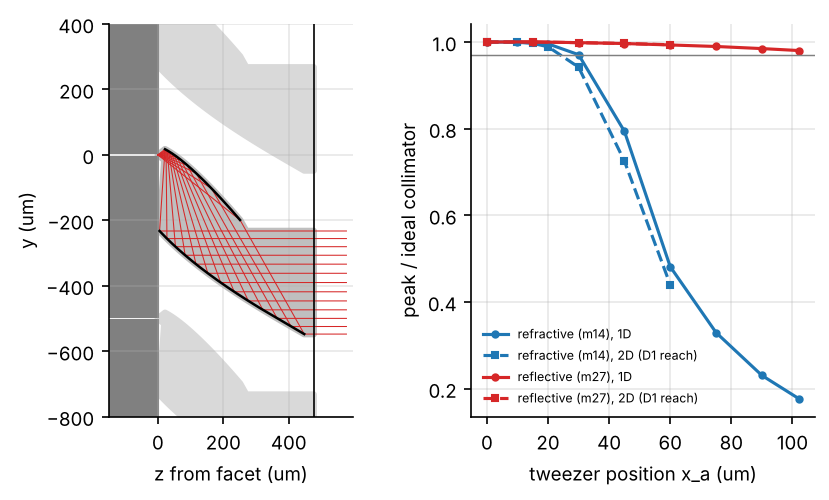
\includegraphics{../results/m27_figure.png}

\emph{Left: y-z section of the adopted block, from the facet (origin) to
the flat exit face, with rays every 6.4 deg in the glass. Grey: the
light regions, with 10 um margin, of the blocks of the neighbouring
chips at +/-0.5 mm. Dark grey: the chips (z \textless{} 0). Right: peak
of a tweezer at x\_a relative to an ideal collimator at the same s\_x,
for the refractive (m26) and reflective (m27) designs; 1D to the slit
edge, 2D within the 67 um reach of the D1 engine of the 2D model.}

\hypertarget{103-the-independent-check}{%
\subsection{10.3 The independent
check}\label{collimator-103-the-independent-check}}

We traced the adopted design through spline fits of the two mirror
curves:

\begin{itemize}
\tightlist
\item
  in 3D, with rays launched with k\_x (not with the effective index);
\item
  with the vector law of reflection;
\item
  with the optical path taken as n times the 3D length.
\end{itemize}

The phase of the k\_x = k0 s\_x component (path minus s\_x x\_exit) is
flat to below 2e-12 waves at s\_x = 0, 0.1, 0.2, 0.312 and 0.355. The
exit height equals f s n / n\_eff to 2e-10, the exit tilt is below 5e-11
rad, and the 2D effective-index lens map used by the wave model agrees
with the 3D trace to 1e-12 waves (\texttt{m27\_trace}). The refractive
design, by contrast, carries 0.30 / 1.18 / 2.86 / 3.67 waves p-v at the
same s\_x. Unit tests cover the same checks.

\hypertarget{104-performance}{%
\subsection{10.4 Performance}\label{collimator-104-performance}}

\textbf{On axis (s\_x = 0)} (\texttt{m27\_wave}):

\begin{itemize}
\tightlist
\item
  The design reproduces the ideal lens in glass and the refractive
  design to four digits: peak per guided power 1.10 relative to the
  ideal lens in air at beta = 0.7 um, y FWHM 1.35 um, crosstalk 4.0e-4 /
  8e-5 at 3 / 4 um.
\item
  With the mirror losses of real coatings, computed from the Johnson \&
  Christy constants of silver and gold (SOURCE, interpolated to 1064.4
  nm: Ag 0.04 + 7.61i, Au 0.26 + 6.97i), the mirror pair reflects:

  \begin{itemize}
  \tightlist
  \item
    99.6\% with M1 silvered and M2 used in TIR;
  \item
    98.2\% with M1 gold.
  \end{itemize}
\item
  The power per 1.2 mK tweezer is 57.7 mW (silver) or 58.5 mW (gold),
  against 57.4 mW for the refractive design with ideal AR coatings.
\item
  Real silver films reflect less than the bulk-quality constants imply
  {[}REF?{]}.
\end{itemize}

\textbf{Across the row} (\texttt{m27\_skew}, effective-index trace
verified above, downstream relay ideal):

{\footnotesize
\begin{longtable}[]{@{}>{\raggedright\arraybackslash}p{0.152\dimexpr(\linewidth-10\tabcolsep)\relax}>{\raggedright\arraybackslash}p{0.183\dimexpr(\linewidth-10\tabcolsep)\relax}>{\raggedright\arraybackslash}p{0.183\dimexpr(\linewidth-10\tabcolsep)\relax}>{\raggedright\arraybackslash}p{0.256\dimexpr(\linewidth-10\tabcolsep)\relax}>{\raggedright\arraybackslash}p{0.226\dimexpr(\linewidth-10\tabcolsep)\relax}@{}}
\toprule\noalign{}
x\_a (s\_x) & peak, reflective: 1D (2D) & peak, refractive: 1D (2D) &
crosstalk at 4 um, reflective / refractive & comb at the far row: loss,
reflective \\
\midrule\noalign{}
\endhead
\bottomrule\noalign{}
\endlastfoot
0 & 1.000 (1.000) & 1.000 (1.000) & 8.4e-5 / 8.4e-5 & 4.8e-3 \\
30 um (0.104) & 0.999 (0.999) & 0.971 (0.942) & 8.4e-5 / 3.0e-3 &
4.9e-3 \\
45 um (0.156) & 0.997 (0.997) & 0.794 (0.725) & 8.6e-5 / 8.2e-3 &
5.0e-3 \\
60 um (0.208) & 0.993 (0.994) & 0.481 (0.440) & 9.0e-5 / 6.9e-3 &
5.1e-3 \\
90 um (0.312) & 0.985 & 0.231 & 9.7e-5 / 9.0e-3 & 5.4e-3 \\
102 um (0.355, slit edge) & 0.980 & 0.177 & 1.0e-4 / 8.6e-3 & 5.5e-3 \\
\end{longtable}
}

Peaks are relative to an ideal collimator of focal length 175 um at the
same s\_x. The remaining 1.5\% at 90 um is the 2.4\% longer focal length
(a slightly wider stripe at S); relative to its own centre the
reflective tweezer keeps 0.990 at 90 um. The y centroid does not move
(below 1e-11 nm), because the mapping stays antisymmetric.

The 2D model covers \textbar x\_a\textbar{} \textless= 60 um only. Its
engine (D1, 128 ports) cannot place a tweezer beyond about 67 um for any
collimator; the 2D values m26 reported at 75 and 90 um are outside the
model (Corrected in \texttt{docs/megascale.md}, Sec. 12).

Hence one engine serves its whole segment: \textbar x\_a\textbar{}
\textless= 90 um, and in 1D to the slit edge. No common focus offset is
needed.

\textbf{Tolerances} (\texttt{m27\_tolerance}):

\begin{itemize}
\tightlist
\item
  Facet decentre and focus behave as for the refractive design: 0.973 at
  0.1 um decentre, 0.995 at 0.5 um focus and 0.977 at 1 um. The decentre
  tolerance remains a property of the facet.
\item
  Exact traces of a displaced source agree with the first-order model of
  the wave model to 1e-4 waves rms (0.2 um decentre) and 3e-4 waves rms
  (0.5 um focus).
\item
  The mirrors are about twice as sensitive to form error as the
  refractive surfaces.
\end{itemize}

{\small
\begin{longtable}[]{@{}>{\raggedright\arraybackslash}p{0.358\dimexpr(\linewidth-6\tabcolsep)\relax}>{\raggedright\arraybackslash}p{0.400\dimexpr(\linewidth-6\tabcolsep)\relax}>{\raggedright\arraybackslash}p{0.242\dimexpr(\linewidth-6\tabcolsep)\relax}@{}}
\toprule\noalign{}
form error, rms (correlation 20 um / 60 um) & reflective, adopted: mean
peak (10th percentile) & refractive (m14) \\
\midrule\noalign{}
\endhead
\bottomrule\noalign{}
\endlastfoot
5 nm & 0.996 (0.993) / 0.998 (0.996) & \\
10 nm & 0.988 (0.983) / 0.989 (0.981) & 0.995 (0.992) / 0.997 (0.994) \\
20 nm & 0.936 (0.902) / 0.957 (0.921) & 0.984 (0.970) / 0.987 (0.968) \\
50 nm & 0.70 (0.54) / 0.79 (0.67) & 0.916 (0.880) / 0.920 (0.823) \\
\end{longtable}
}

Hence the two mirrors need \textless= 10 nm rms for \textless= 2\% loss,
against about 20 nm for the refractive surfaces. The TIR variant, with
lower sensitivity, gives 0.989 / 0.956 at 10 / 20 nm (20 um
correlation).

\textbf{x axis} (\texttt{m27\_xaxis}). The folded glass path changes the
x geometry, but the effect is small.

\begin{itemize}
\tightlist
\item
  \textbf{Geometry.} The glass path of the axial ray is 749 um. The x
  slit plane lies 6.72 mm from the facet, and the virtual plane S lies
  0.29 mm behind it (the chief-ray construction of a folded system).
\item
  \textbf{Comb.} The comb therefore starts 7.51 mm from S, and the far
  row of a 32-row comb sits at 23.5 mm (23.0 mm with the refractive
  collimator). There the comb loses 4.8e-3 at x\_a = 0 and 5.5e-3 at the
  slit edge, with crosstalk at 4 um of 1.1e-4.
\item
  \textbf{Slab phase.} After its defocus is absorbed by placing the x
  lens, the glass slab adds 0.47 waves p-v of higher-order phase in s\_x
  (refractive: 0.17). Before recalibration it costs D1 tweezers at +/-60
  um less than 3e-4 in peak and 1.4 nm in position; after recalibration,
  nothing measurable.
\end{itemize}

\hypertarget{105-polarisation}{%
\subsection{10.5 Polarisation}\label{collimator-105-polarisation}}

The refractive collimator works below total internal reflection, with
real Fresnel coefficients, so it adds no s-p phase and no circular
polarisation (DERIVED). Mirrors do add one. The TE field of the chip (E
along x) is pure s-polarisation for s\_x = 0, so nothing happens on
axis. For s\_x != 0 the plane of incidence tilts, the field gains a p
component, and the s-p phase of the reflection mixes the two.

We traced the field through both mirrors in 3D (\texttt{m27\_pol}):

\begin{itemize}
\tightlist
\item
  launch: TE, the x unit vector projected transverse to each ray;
\item
  reflection: Fresnel coefficients of each coating, in a convention
  checked against a perfect conductor;
\item
  metric 1, the cross-polarised power at the centre of the tweezer: the
  coherent pupil sum, weighted by the facet far field;
\item
  metric 2, its degree of circular polarisation V.
\end{itemize}

Perfect mirrors give neither (below 1e-26). The coatings do. Their s-p
phase departs from that of a perfect mirror (the excess retardance) as
follows:

\begin{itemize}
\tightlist
\item
  silver in fused silica: 6 deg at 30 deg incidence, 31 deg at 60 deg,
  68 deg at 75 deg;
\item
  TIR: 142 to 159 deg between 45 and 75 deg, close to a half-wave.
\end{itemize}

{\small
\begin{longtable}[]{@{}>{\raggedright\arraybackslash}p{0.395\dimexpr(\linewidth-10\tabcolsep)\relax}>{\raggedright\arraybackslash}p{0.218\dimexpr(\linewidth-10\tabcolsep)\relax}>{\raggedright\arraybackslash}p{0.129\dimexpr(\linewidth-10\tabcolsep)\relax}>{\raggedright\arraybackslash}p{0.129\dimexpr(\linewidth-10\tabcolsep)\relax}>{\raggedright\arraybackslash}p{0.129\dimexpr(\linewidth-10\tabcolsep)\relax}@{}}
\toprule\noalign{}
coating (adopted layout unless stated) & x\_a = 30 um: cross-pol / V &
60 um & 90 um & 102 um \\
\midrule\noalign{}
\endhead
\bottomrule\noalign{}
\endlastfoot
perfect mirrors & 0 / 0 & 0 / 0 & 0 / 0 & 0 / 0 \\
M1 silver, M2 TIR & 1.0e-2 / -0.013 & 4.2e-2 / -0.026 & 9.6e-2 / -0.039
& 0.12 / -0.045 \\
M1 gold, M2 TIR & 1.0e-2 / -0.009 & 4.2e-2 / -0.018 & 9.5e-2 / -0.027 &
0.12 / -0.031 \\
both silver & 1.6e-3 / -0.072 & 6.7e-3 / -0.146 & 1.6e-2 / -0.223 &
2.1e-2 / -0.256 \\
TIR variant, both TIR & 3.3e-3 / +0.093 & 1.3e-2 / +0.185 & 2.9e-2 /
+0.277 & 3.8e-2 / +0.313 \\
lossless coating, excess retardance 2 deg on both & 1.5e-5 / -0.008 &
5.8e-5 / -0.015 & 1.3e-4 / -0.023 & 1.6e-4 / -0.026 \\
same, 5 deg & 9.2e-5 / -0.019 & 3.6e-4 / -0.038 & 8.0e-4 / -0.056 &
1.0e-3 / -0.064 \\
same, 10 deg & 3.7e-4 / -0.038 & 1.4e-3 / -0.075 & 3.2e-3 / -0.111 &
4.1e-3 / -0.125 \\
\end{longtable}
}

Three points follow.

(i) The circular component grows linearly with x\_a and with the excess
retardance, by about 0.011 per degree at x\_a = 90 um (two mirrors).

(ii) The layout does not help. With two silver mirrors, all 290 passing
layouts give \textbar V\textbar{} = 0.20 to 0.23 at 90 um
(\texttt{m27\_poltrade}). The least form-sensitive layouts have the
larger incidence angles, so polarisation and form tolerance do not trade
usefully.

(iii) The coating does. Using M2 in TIR, its near half-wave retardance
largely cancels the ellipticity of the silver or gold on M1. The
circular component falls to \textbar V\textbar{} \textless= 0.04
(silver) or 0.03 (gold) at 90 um, but the polarisation is then rotated
as a whole, by about 18 deg at 90 um (cross-polarised power 0.096). This
is the adopted configuration.

For alkali ground states (J = 1/2) the light shift depends on the
circular component (vector shift, proportional to V m\_F) but, apart
from a small hyperfine-induced tensor part, not on the direction of
linear polarisation. The rotation is therefore benign to first order,
and V is the figure that matters. For m\_F = 0 clock states the
first-order vector shift vanishes. We have not set a criterion for V for
the qubit encoding and bias field used in transport {[}VALUE?{]}.

If a lower V is needed, there are two options:

\begin{itemize}
\tightlist
\item
  a coating with an excess retardance of about 2 deg or less over 28 to
  77 deg on both mirrors, giving \textbar V\textbar{} \textless= 0.023
  and almost no rotation;
\item
  a compensating retarder at the x slit plane, where x encodes s\_x.
\end{itemize}

Neither is designed here. The comb teeth add a further reflection at 45
deg for half of the stacks, which we did not include.

\hypertarget{106-limits-and-next-steps}{%
\subsection{10.6 Limits and next
steps}\label{collimator-106-limits-and-next-steps}}

The trace is exact for cylindrical mirrors, and the wave model is 1D,
with 2D checks to 60 um. Coatings and TIR enter through their Fresnel
coefficients only, with no thin-film stack designed. The downstream
relay, the comb teeth (another reflection at 45 deg) and the objective
are ideal or not modelled for s\_x != 0. Polarisation is evaluated at
the pupil, before the objective.

Next steps:

\begin{itemize}
\tightlist
\item
  (i) a coating with small s-p retardance over 28 to 77 deg on M1, or a
  layout with smaller incidence angles (Sec. 10.5);
\item
  (ii) a fabrication route for a 0.48 mm fused-silica block with two
  freeform mirrors at \textless= 10 nm rms (diamond- turned moulds,
  grey-scale lithography or two-photon printing followed by reflow
  {[}REF?{]}), registered to each other to the precision the
  construction assumes;
\item
  (iii) a tolerance Monte Carlo of the block with all errors combined;
\item
  (iv) the polarisation criterion for the qubit encoding used in
  transport.
\end{itemize}

\hypertarget{verification-notes}{%
\section{Verification notes}\label{collimator-verification-notes}}

{\footnotesize
\begin{longtable}[]{@{}>{\raggedright\arraybackslash}p{0.230\dimexpr(\linewidth-8\tabcolsep)\relax}>{\raggedright\arraybackslash}p{0.129\dimexpr(\linewidth-8\tabcolsep)\relax}>{\raggedright\arraybackslash}p{0.101\dimexpr(\linewidth-8\tabcolsep)\relax}>{\raggedright\arraybackslash}p{0.539\dimexpr(\linewidth-8\tabcolsep)\relax}@{}}
\toprule\noalign{}
value & location & type & pointer \\
\midrule\noalign{}
\endhead
\bottomrule\noalign{}
\endlastfoot
designs, limits, geometry & Sec. 1, 2 & SIM & results/m14\_designs.json
(review) \\
facet R, T, capture & Sec. 1, 3 & SIM &
results/m14\_facet\_meep\_\{air,glass\}.json (review) \\
wave-model table & Sec. 1, 4 & SIM & results/m14\_wave.json (review) \\
tolerances, exact checks & Sec. 1, 5 & SIM & results/m14\_tolerance.json
(review) \\
form Monte Carlo & Sec. 5 & SIM & results/m14\_form.json (24 samples per
point; review) \\
x lens & Sec. 6 & SIM & results/m14\_xlens.json (review) \\
power plan, fibres, offsets & Sec. 1, 8 & DERIVED &
results/m14\_plan.json \\
parameter scan of the Weierstrass design & Sec. 2 & SIM &
results/m14\_scan.json \\
2D check of the adopted design (1.107) & Sec. 1 & SIM & run in session,
not stored \\
n(SiO2) 1.4496 & throughout & SOURCE & Malitson (picsim/materials.py) \\
n = 1.8, R 80 um, gap 10 um, T 250 um, AR coatings & Sec. 2, 4 & CHOICE
& design choices \\
CTE Si 2.6e-6/K, fused silica 0.55e-6/K & Sec. 7 & RECALLED & verify \\
20 MW/cm\^{}2 facet cap & Sec. 8 & CHOICE & m6 (no damage threshold
found) \\
\end{longtable}
}

\textbar{} reflective collimator: scan, construction, selection
\textbar{} Sec. 10.2 \textbar{} SIM \textbar{} results/m27\_scan.json
(review) \textbar{} \textbar{} 3D trace: W, mapping, effective-index
check \textbar{} Sec. 10.3 \textbar{} SIM \textbar{}
results/m27\_trace.json \textbar{} \textbar{} wave model, mirror
reflectance, power \textbar{} Sec. 10.4 \textbar{} SIM \textbar{}
results/m27\_wave.json (review) \textbar{} \textbar{} skew, comb at the
far row \textbar{} Sec. 10.4 \textbar{} SIM \textbar{}
results/m27\_skew.json, results/m27\_skew\_summary.json (review)
\textbar{} \textbar{} tolerances, form Monte Carlo \textbar{} Sec. 10.4
\textbar{} SIM \textbar{} results/m27\_tolerance.json (24 samples per
point; review) \textbar{} \textbar{} x geometry, slab phase \textbar{}
Sec. 10.4 \textbar{} SIM \textbar{} results/m27\_xaxis.json (review)
\textbar{} \textbar{} polarisation, coating trade \textbar{} Sec. 10.5
\textbar{} SIM \textbar{} results/m27\_pol.json,
results/m27\_poltrade.json (review) \textbar{} \textbar{} n(Ag), n(Au)
at 1064.4 nm \textbar{} Sec. 10.4, 10.5 \textbar{} SOURCE \textbar{}
Johnson \& Christy, Phys. Rev. B 6, 4370 (1972),
doi:10.1103/PhysRevB.6.4370; refractiveindex.info tables retrieved
2026-11-09, interpolated \textbar{} \textbar{} 0.5 mm length limit, 10
um clearance, 20 um radius limit \textbar{} Sec. 10.2 \textbar{} CHOICE
\textbar{} design choices \textbar{}

Open placeholders: {[}REF?{]} UV-adhesive shrinkage and creep at the 0.1
um level; {[}REF?{]} placement accuracy of two-photon-printed
micro-optics on chip facets; {[}VALUE?{]} CW power handling of
acousto-optic shifters at 3 W, 1064 nm; {[}VALUE?{]} available
single-frequency 1064 nm power at 40 to 55 W; {[}REF?{]} reflectance of
deposited silver on fused silica at 1064 nm; {[}REF?{]} fabrication of
freeform glass micro-mirrors at \textless= 10 nm rms; {[}VALUE?{]}
tolerable circular polarisation of the transport tweezers.
